\documentclass[letter,twocolumn]{article}
\usepackage{listings}
\usepackage{graphicx}
\usepackage{caption}
\usepackage{pgf}
\usepackage{tikz}
\usepackage{dblfloatfix}
\usepackage{fixltx2e}
\setlength{\footskip}{20pt}

\usetikzlibrary{arrows,positioning} 
\tikzset{
    %Define standard arrow tip
    >=stealth',
    %Define style for boxes
    punkt/.style={
           rectangle,
           rounded corners,
           draw=black, very thick,
           text width=6.5em,
           minimum height=2em,
           text centered},
    % Define arrow style
    pil/.style={
           ->,
           thick,
           shorten <=2pt,
           shorten >=2pt,}
}
%\usepackage[left=.75in,right=.75in,top=1in,bottom=1in]{geometry}

\definecolor{mygreen}{rgb}{0,0.6,0}
\definecolor{mygray}{rgb}{0.5,0.5,0.5}
\definecolor{mymauve}{rgb}{0.58,0,0.82}

\lstset{ %
  backgroundcolor=\color{white},   % choose the background color; you must add \usepackage{color} or \usepackage{xcolor}
  basicstyle=\footnotesize,        % the size of the fonts that are used for the code
  breakatwhitespace=false,         % sets if automatic breaks should only happen at whitespace
  breaklines=true,                 % sets automatic line breaking
  captionpos=b,                    % sets the caption-position to bottom
  deletekeywords={...},            % if you want to delete keywords from the given language
  escapeinside={\%*}{*)},          % if you want to add LaTeX within your code
  extendedchars=true,              % lets you use non-ASCII characters; for 8-bits encodings only, does not work with UTF-8
  frame=single,                    % adds a frame around the code
  keepspaces=true,                 % keeps spaces in text, useful for keeping indentation of code (possibly needs columns=flexible)
  language=Octave,                 % the language of the code
  morekeywords={*,...},            % if you want to add more keywords to the set
  numbers=left,                    % where to put the line-numbers; possible values are (none, left, right)
  numbersep=5pt,                   % how far the line-numbers are from the code
  numberstyle=\tiny\color{mygray}, % the style that is used for the line-numbers
  rulecolor=\color{black},         % if not set, the frame-color may be changed on line-breaks within not-black text (e.g. comments (green here))
  showspaces=false,                % show spaces everywhere adding particular underscores; it overrides 'showstringspaces'
  showstringspaces=false,          % underline spaces within strings only
  showtabs=false,                  % show tabs within strings adding particular underscores
  stepnumber=1,                    % the step between two line-numbers. If it's 1, each line will be numbered
  tabsize=2,                       % sets default tabsize to 2 spaces
  title=\lstname                   % show the filename of files included with \lstinputlisting; also try caption instead of title
}


\usepackage{fancyhdr}
\pagestyle{fancy}

\setcounter{secnumdepth}{2}

\setlength\headheight{24pt}
\setlength\headsep{12pt}
\setlength\footskip{12pt}
\setlength{\parindent}{0pt} 
\setlength{\parskip}{2ex}

\lhead{\textbf{iDcDashboard}} % center: document title
\rhead{\textbf{David Lisuk}} % header right: name & student ID
\cfoot{\thepage}
\title{iDcDashboard -- An Interactive Plotting Tool for Big Data}
\author{David Lisuk}
\date{\today}
\begin{document}
\bibliographystyle{plain}
\twocolumn[\begin{@twocolumnfalse}
\maketitle

\begin{abstract}
This paper describes the design and implementation of the iDcDashboard system, an iPython Notebook widget for exploratory visualization of large data sets. 
iDcDashboard exposes a simple to use API for the creation of interactive visualizations.
The layered design of the system allows for easy extensibility of the front and back ends of the system without knowledge of the iPython Notebook widget interface.
Large data sets are handled through the use of server side data sampling, and drilling down into data is supported via resampling of data within a selected data subset.
Performance tests are used to show that plotting of both both local and remote datasets are within acceptable time limits.
\end{abstract}
\vspace{0.25in}
\end{@twocolumnfalse}]

\section{Introduction}%1 page

The modern deluge of data has lead to the need for tools and techniques to analyze very large sets of data.
This has spurned the development of novel data processing paradigms\cite{dean2008mapreduce}\cite{zaharia2010spark}, analysis algorithms\cite{bekkerman2011scaling}, and data management systems\cite{tauro2012comparative}.
However, specialized tools for exploratory data analysis are few and far between, leading to the use of ad hoc hacks.
In particular visual exploration of large data sets is a difficult endeavor with existing tools leading analysts to manually select and sample data, create static visualizations, and iterate.
This slows the data analysis process down and provides ample opportunity for improvement.
The aim of this paper is to improve this situation by integrating interactive plotting directly into iPython Notebook\cite{perez2013open}, a web based Python environment targeted toward data analysis.

The remainder of this paper is organized into five sections.
Section 2 elaborates on the exploratory analysis problem and the goals of this project.
Section 3 introduces the iDcDashboard system, our solution for exploratory analysis.
Section 4 addresses scaling of iDcDashboard to larger data sets.
Section 5 evaluates the performance on various sized data sets.
Section 6 concludes and discusses future directions.

\section{Exploratory Analysis}

Prior to modeling any dataset, an analyst must look at the data to find and fix idiosyncrasies and to plan further analysis technique.
While statistical summaries serve a purpose in this endeavor, the human eye is far better at processing visual information.
Thus, exploratory visualizations are a critical step in the analysis pipeline.
However, performing exploratory analysis on a modern dataset, often terabyte and beyond scale, presents a number of unique challenges which have yet to be addressed in a single publicly available system.

A critical issue in visualizing big data is the limited screen real estate relative to the number of unique records.
Thus, a primary goal must be to efficiently utilize screen space.
Although this could be done by allowing the creation of artful information displays as seen in Tufte's work\cite{Tufte:1986:VDQ:33404} and the d3 gallery\cite{d3galery}, such displays require a design effort beyond what is attainable for a single throwaway exploratory graphic.
A common technique is for an analyst to down sample the data such that it can be effectively visualized in the prescribed screen space.  
This idea can be extended by allowing the user to modify the plots by selecting regions of interest and then always keeping a good suitable sample within the selected region displayed.  
Thus, the effective utilization of screen real estate is through exploitation of the interactive nature of the computer.
However, human nature being what it is, adoption of this technique requires high responsiveness and easy modification.

While the responsiveness goal dictates that data must be local to the visualizations, no workstation is capable of holding the largest datasets analyzed today.
Thus, the visualization must be backed by a data provider capable of handling the scale.
Ideally, the data provided to the client should be informed by the interactions of the user, leading to more client memory being used to hold actively viewed data and less on holding cold data.

A primary goal of exploratory analysis is the discovery and cleansing of data impurities or relationships that are incompatible with the planned modeling technique.
Visualizations are needed prior and after the data processing to verify proper cleansing.
Thus, switching between a processing environment and visualization environment is incompatible with exploratory analysis.
This dictates that the visualizations be tightly integrated with an existing data processing system.
Tight integration includes simple and idiomatic API design for the creation of visualizations.

Individually, these issues have been solved; however, no single public system brings them all together.
The interactive plotting package dc.js\cite{dcjs} provides responsive interactive visualizations suitable for exploratory analysis.
However, dc.js requires extensive knowledge of JavaScript to utilize and is only a client side tool with no ability to connect to backing data stores.
iPython Notebook also provides an integrated visualization and processing environment and can connect to any data store; however, its interactive plotting features are nascent and again suffer when trying to scale.
Thus, it is believe that the best solution is to integrate dc.js and iPython Notebook to make a single exploratory visualization system.

\section{iDcDashboard}% 2 pages

Through the use of iPython Notebook's widget facility, dc.js is able to be integrated into standard iPython Notebooks to create the iDcDashboard system.
The iDcDashboard is a collection of interactive plots over a shared tabular dataset.
By using a fairly simple idiomatic Python API, interactive plots can be connected to an arbitrary data backend.
Built in functionality allows client side data selection to request high resolution samples of areas of interest.
A layered system architecture allows for easy extension of the frontend and backend without having to worry about the communication between the two.

\subsection{iPython Notebook Widget}

iPython Notebook\cite{perez2013open} is the ideal environment for exploratory analysis since it allows literate programming within the Python programming language.
Structured markdown text, graphics, Python code, and HTML/JavaScript all reside within a single interface, allowing the creation of a document showing the complete data analysis process. 
Due to these advantages, iPython Notebook has become one of the main environments for analytic work.

A powerful feature of iPython Notebooks is the widget facility.
A widget is an interactive HTML/JavaScript client displayed within an iPython Notebook which communicates with a server side Python object.
Although they are a recent innovation, several interesting examples pointing to their future importance have popped up throughout the web\cite{widget}.

The iDcDashboard fits well into the widget model since it has a distinct client (the interactive visualizations) and backend (the data provider).
Communication between the two sides in a widget is provided by the creation of shared variables which can be read and written from either side without any protection or synchronization.
In iDcDashboard, a convention that each shared variable will either be written by the Python or JavaScript and read by the other side is adopted.
Callback functions are registered on the reading side so the reader would be notified whenever a change was made to each variable and the appropriate action could be taken.
With this convention the communication can be thought of as a pipe and thus these shared variables are refered to as pipes throughout the rest of this paper.

\subsection{System Architecture}
\begin{figure}[htb]
	\begin{center}
	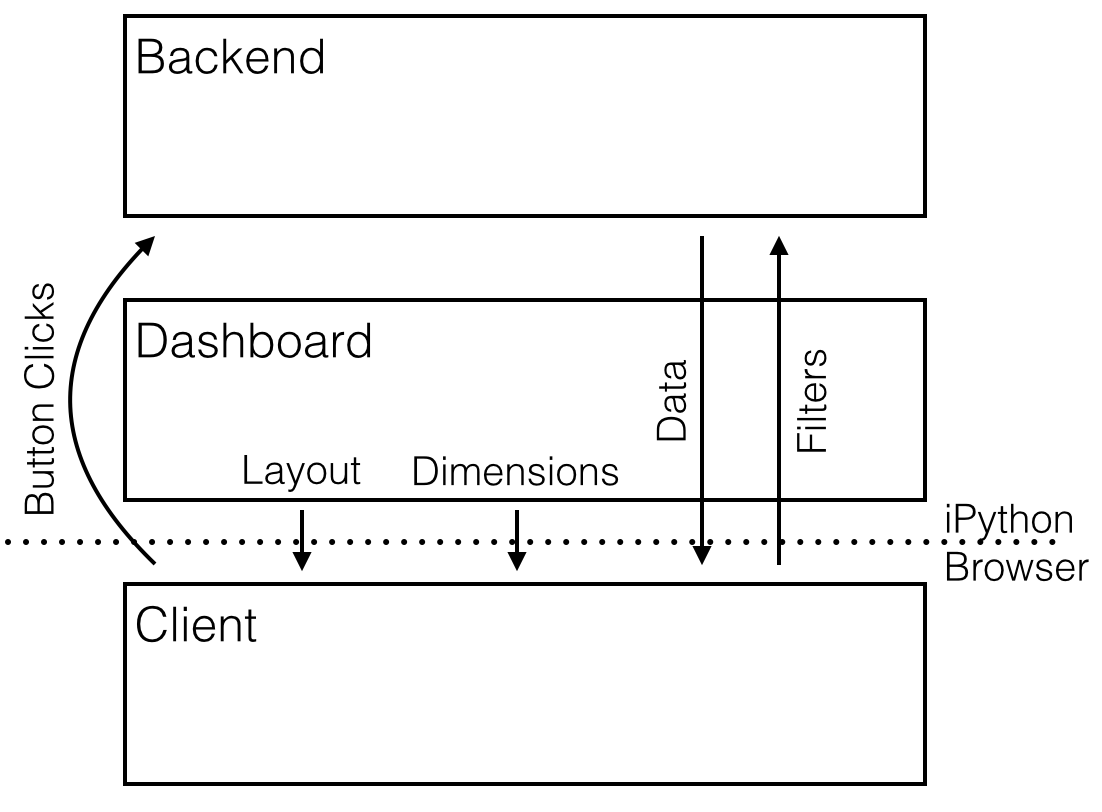
\includegraphics[width=3in]{figs/dataflow.png}
	\end{center}
	\caption{Data flow within the iDcDashboard system}\label{fig:system_flow}
\end{figure}

To ease implementation and extensibility, the iDcDashboard is segmented into three layers: the backend, the dashboard, and the client.
These three layers communicate through four pipes as seen in Figure \ref{fig:system_flow}.

The dashboard is the central layer and serves two main purposes.
First, it exposes a simple Python interface to configure the browser-based client layer.
Second, it provides an interface for two way communication between the client and the backend.
This layer is the main layer a user will program on.

The client manages the visualizations and a data cache.
Each plot type implements a simple JavaScript object interface.
This allows the addition of new plot types without any backend coding or understanding of the system as a whole.

The backend manages the iPython local data cache, connects to remote data providers, and sends data to the client through the dashboard.
New data providers or data processing methods can be added through the implementation of a simple interface.

We now go into detail on each of these three layers individually.

\subsubsection{Dashboard}\label{sec:dashboard}

The dashboard class serves as the middleware between the backend and the client.
Upon construction, the object creates and configures the client and registers itself with the backend.
Once constructed, it exposes two communication pipes which are used for communication between the backend and the client.

The constructor of the dashboard accepts three parameters: the backend object, a list of dimensions to create, and a list of rendering directives.
Details of the dimension and rendering directives themselves will be discussed in Section \ref{sec:api}; however, they are best thought of as a domain specific language for the generation of the client's JSON configuration discussed in Section \ref{sec:client}.
After configuring the client, the dashboard registers itself with the backend and renders an optional toolbar provided by the backend (this toolbar provides a direct user interface to the backend).
Once constructed, the main function of the dashboard is to provide two pipes between the backend and the client.

The \emph{data} pipe is used by the backend to override the data in the client with a new set of data.  
The pipe uses a JSON blob containing a single JList of JObjects.
Since the system is only designed to handle tabular datasets, the JObjects are expected to be flat, that is only contain strings or numerics for values.
To ease backend programming, the dashboard also accepts Pandas DataFrame (a common Python abstraction for tabular data) or Python lists of dictionaries which it will be converted to the correct JSON blob format.

The \emph{filter} pipe is used by the client to inform the backend of the data region currently zoomed in on 
Two kinds of filters are supported: set inclusion and numeric range filters.
A set inclusion filter is a list of all values which the analyst has selected (\emph{e.g.,} on a mapping application a list of states the user is analyzing may be passed).
Range filters are min max pairs specifying a numeric range of data the analyst has selected.
When multiple filters are applied to the same field, the union of the rows accepted by each filter is accepted.
The dashboard translates all filters to use field names and formats understood by the backend rather than the client.

\subsubsection{Client}\label{sec:client}

The client is a collection of JavaScript objects which work together to render the desired plots.
The key components are the layout engine,  the plotting code, and the data manager.

The layout engine interprets a layout configuration provided in JSON format.
The JSON configuration is a JArray of JObjects describing objects to render.
All objects to be rendered have a type field which specifies which object to render.
There are two distinct classes of objects which can be rendered: layers and plots.
A layer creates a new div as wide as the rendering area, which has a specified height.
Each layer can hold any number of plots side by side while layers are vertically stacked.
All plots will be rendered into the last defined layer.
An example of this semantic is displayed in Figure \ref{fig:layout}.
Note how the first two plots (the bar and scatter) render within the first layer and the third plot renders in the second layer.
A plot object contains configuration describing the plot, typically the data source it will plot from, the width, and plot type specific configuration directives.
The layout engine creates a div within the previous layer's div and passes it as a target for the plotting code to render onto.

\begin{figure}
\begin{lstlisting}
[{type:layer, height: 300}, 
  {type:bar,  ...},
  {type:scatter, ....},
  {type:layer, height 200},
  {type:row, ...}
]
\end{lstlisting}

\begin{lstlisting}
[
  Layer(300), 
  Plot("bar")..., 
  Plot("scatter")...,
  Layer(200), 
  Plot("row")
]
\end{lstlisting}
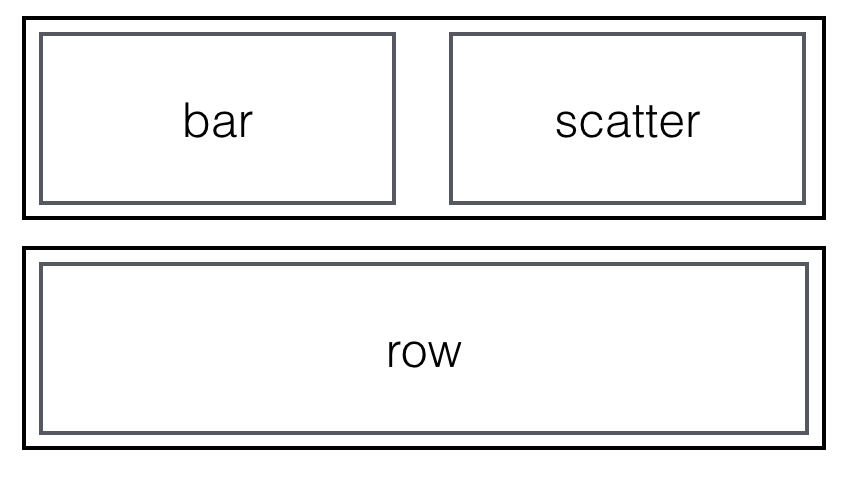
\includegraphics[width=3in]{figs/layout_example.png}
\caption{\emph{(Top)} Example configuration code for client layout engine along with \emph{(Middle)} the Python code to generate said configuration.  Finally \emph{(Bottom)} a diagram showing how the plots will be rendered.}\label{fig:layout}
\end{figure}

While the layout engine creates the divs for laying out plots, the actual plotting is done by specialized classes for each plot type.
The type field of the configuration object is used to look up the specific object get.
All plot objects define {\tt render, set\_data\_source, update\_data, height, and width} methods which are used to control the creation of the object.
In addition to the standard object creation methods, an additional set of plot specific configuration methods can be defined.
We have used this to implement setting of domain and range on x/y coordinate plots, setting axis labels, and other useful options.
In the current system, all plottable objects come from the dc.js package but this interface in general enough that other plotting libraries or even raw HTML generation code could go in this framework.

Finally, the data manager holds the data passed from the server and connects plots to plottable data.
To hold the data, Square's Crossfilter.js\cite{crossfilter} library is used.
Crossfilter provides a data structure which holds JSON records and allows for quick and efficient sorting and selection to support the interactive plots.
To support this, Crossfilter creates \emph{dimension} and \emph{group} objects on the data.
A dimension converts the arbitrary records into a plottable series of either a single data value per row or an ($x$,$y$) pair of values per row.
A group defines a map-reduce function which collects points in a dimension together and then replaces the grouped points with a single value.
A typical use of a group is to create a binned histogram of a dimension by mapping the dimension to a bin and then reducing by counting the number of records in each bin.

The data manager accepts a JSON configuration for creating dimensions/groups and assigns each dimension and group a name.  
This is done by passing a JObject where keys are dimension names and values are another JObject describing the given dimension.
A dimension's JObject contains the JavaScript code for mapping a record to the points and an object describing all the groups in a similar manner as the dimensions.
The data manager then allows referring to a dimension and group by the name ``{\tt cf/(dim name)/(group name)},'' and by default, creates a null group which uses an identity mapping for points and returns the count for each distinct value.

\subsubsection{Backend}\label{sec:backend}

The backend connects to a local or remote data source and chooses which data to send to the client.
Typically, the backend is simply a fa\c{c}ade over a standard data set providing object or a network connection to a remote dataset.  
However, it is possible to create a backend that produces data or performs more complicated data processing tasks.

There are two ways for the user to interact with the backend.
First, the backend exposes a toolbar which is a collection of buttons and form elements which have callback functions into the backend.
This allows the backend to have specialized user interaction such as allowing the user to hint when new data should be sent or modifying the underlying stored values for selected data.
Secondly, every time a filter is modified on a plot the client notifies the backend as described in Section \ref{sec:dashboard}.
Each time either of these events happen the backend can decide to push a new dataset to the dashboard/client as described in \ref{sec:dashboard}.

A very simple backend is the standard {\tt Backend.DF\_Backend} which accepts a Pandas DataFrame and pushes it to the dashboard upon dashboard registration.
This backend never pushes a new data set and is suitable for analysis of small static datasets.
A set of more powerful backends capable of plotting bigger or dynamic datasets is described in Section \ref{sec:bigdata}.
It is expected that most extension and customization of the iDcDashboard system will come in the form of new backends to handle different kinds of data sets and processing work flows.

\subsection{Programming Interface}\label{sec:api}

To use iDcDashboard, the user creates a new instance of the Dashboard object by passing three parameters: the backend, list of dimensions, and layout configuration.

As described in Section \ref{sec:backend}, the backend is a Python object which connects to a dataset the user wishes to analyze.

Dimensions are configured via the Dimension and Group classes which provide automatic generation of the data manager configuration discussed in Section \ref{sec:client}.
An example of the dimension configuration is seen in \ref{fig:simple_example}.
A dimension is either a single column (used for the primary axis on most plots) or a pair of columns (used for (x,y) scatter plots) from the dataset.
A group describes how to compute the secondary axis on single column dimensions.
While simple groups can be specified in pure Python, the nature of groups is that they are client-side processing routines, and thus the ability to write JavaScript functions is exposed.
Default names are assigned to dimensions consisting of the names of the columns used to create the columns seperated by underscores.
For example, if $X$ and $Y$ are two columns, a dimension with just $X$ will be given the name $X$ and a dimension of $X$ and $Y$ will be given the name $X$\_$Y$.
All groups must be manually named.

The configuration of plots is done by passing a list of Layer and Plot objects. 
This provides a Python abstraction over the layout engine JSON configuration described in Section \ref{sec:client}.
The layer constructor accepts a single parameter describing the layer height.
The plot constructor accepts the type of the plot (bar, scatter, and pie are example types) and then uses the builder design pattern of having configuration methods to apply further configuration.
The most important method is the {\tt data\_source} method, which accepts two parameters, the dimension and group (defaults to an neutral group).
Additional methods ({\tt title, width}, etc.) control the formatting of the plot.
In order to support plot specific configuration settings, the {\tt config} method is used.
The {\tt config} method accepts a variable name followed by a list of parameters and is used for plot specific features (domain and range, axis titles, color and size of scatter points, etc).

\begin{figure*}[hb]
\begin{lstlisting}
Dashboard(
  Backend.DF_Backend(data_frame), 
  [
    Dimension("field_1","field_2"),
    Dimension("field_3", name_override = "third field").
      add_group("rounded",Group("function(d){return 20*Math.floor(d/20);}"))
  ],
  [
    Layer(200),
    Plot("scatter").data_source("field_1_field_2").width(400),
    Plot("bar").data_source("third field","rounded").width(400)
  ]
).show()
\end{lstlisting}

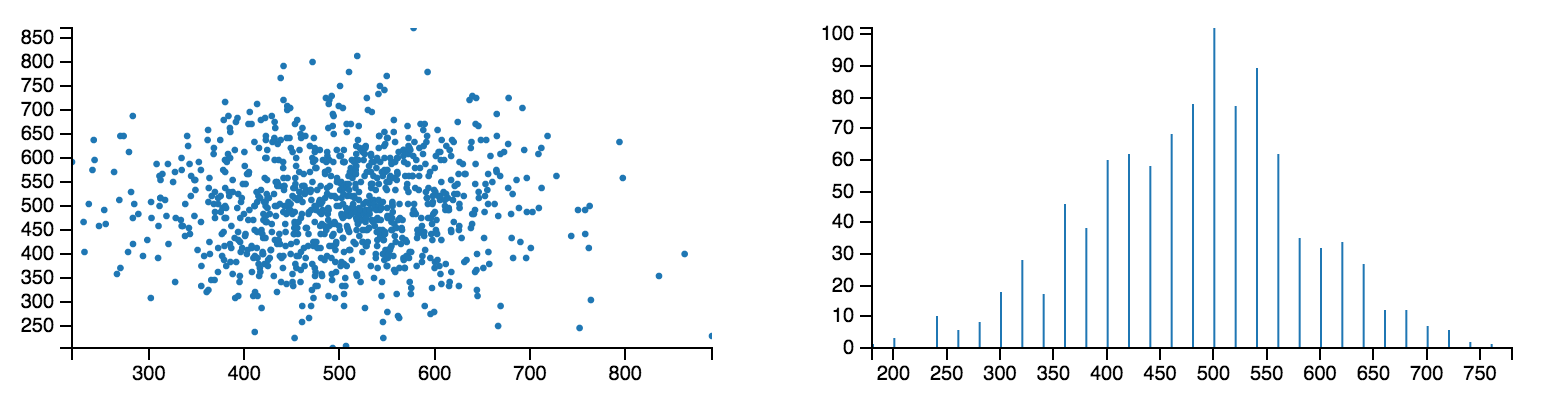
\includegraphics[scale=.63]{figs/screenshot_scatter_bar.png}
  \caption{\emph{Above:} Basic code to create a scatter plot and bar plot of a Pandas DataFrame.  \emph{Below:} the resulting plots.}\label{fig:simple_example}
\end{figure*}

\section{Scaling to Big Data}\label{sec:bigdata}%2 pages
Scaling to large data is handled in two stages.  
First, data small enough to fit in iPython's memory (but not the client's memory) is handled.  The system is then scaled up to larger data by using an Apache Spark cluster as a data store which is accessed through a REST API.  These two solutions will be discussed separately.

\subsection{iPython Resident Datasetets}
In the first stage, the dataset is small enough to fit within iPython's memory as a Pandas DataFrame.
However, the data is either too large to fit in the client memory or is too dense to visualize within a single view.

Upon creation, a sample of about 5000 records is sent to the client.
As the user applies filters to the data, the iPython Notebook adds a sample within the region selected and adds it to the displayed data.
As the user zooms out, the added data is removed and replaced with new data from the new area of interest.
Thus, the user always sees about 5000 points within their data at any scale.

\subsection{Remote Datasets}\label{sec:big_data_remote}

While the first stage of scaling solves the scaling issue to data sets which are loadable in Python, it limits the scale to things that can fit in pandas on a single server.
Larger datasets or streams of data (\emph{e.g.}, Tweet streams) cannot fit into this model since they cannot fit into a single server's memory and often are changing in nature and thus cannot be put into a static Pandas DataFrame.
This problem is solvable by creating custom backend objects for the users specific needs.
The {\tt HTTPS\_Backend} coupled with the Restful RDD project allows arbitrarily large data sets to be visualized in the iDcDashboard.

Data is stored within a Apache Spark RDD containing record objects.  A webservice was written in Scala using the Scalatra web framework which connects to the Spark RDD and exposes a restful API for acquiring samples of the data suitable for pushing to the front end.  
The Python backend initially requests a data set small enough to fit within its memory and typically acts in the same way as with any iPython resident dataset.
However, as the resident dataset fails to fully populate the client, additional data in the area of interest is pulled from the remote dataset.
Thus, this behavior is similar to a three level cache with a large but slow remote data store, a fast client data store, and a medium speed Python data store.

The REST API used in this system has the following interface:
\begin{enumerate}
	\item The dashboard makes a POST request containing the filters and number of records to pull.
	\item The server responds with a unique dataset id where it will store the results.
	\item The dashboard makes a GET request for the dataset id every second. 
	The server responds with HTTP 202:Accepted if data is not ready or HTTP 200:OK and the data if it is ready.
\end{enumerate}
Once the data is downloaded, it can be pushed to the client at the backend's leisure.

\section{Performance Evaluation}%1 page

To evaluate performance, the time to resample a large dataset and the time to plot the dataset are the most critical.
The performance of these two actions is evaluated on both a local and a remote backend.

\subsection{Local Backend}

The first experiment tests the performance on a local dataset.
The experiment uses a set of NOAA US historical weather data containing 4.2 million temperature measurements, which stores to a 300 MB file.
The weather dashboard is configured with eight distinct plots: a scatter plot of measurement latitude/longitude, a pie chart of measurements state, a scatter plot of temperature/day of year,  a histogram of temperature, a histogram of day of year binned into 5 day chunks, a histogram of year binned to nearest decade, and a pie chart of quarter of year.
A screenshot of this dashboard can be seen in the appendix.

To evaluate performance, the time between clicking the resample button until the data has completed pushing to the client and the time from the client receiving the data until the plots have finished rerendering are each measured.
This test is conducted with exponentially increasing sample sizes of 100, 1000, 10000, 100000 data points 5 times per sample size.
At the sample size of 100 and 1000 the tools were all very responsive; however, at 10,000 responsiveness was slow but acceptable.
At 100,000 data points the GUI was extremely difficult to use and could be considered unusable.

\begin{figure}
\begin{center}
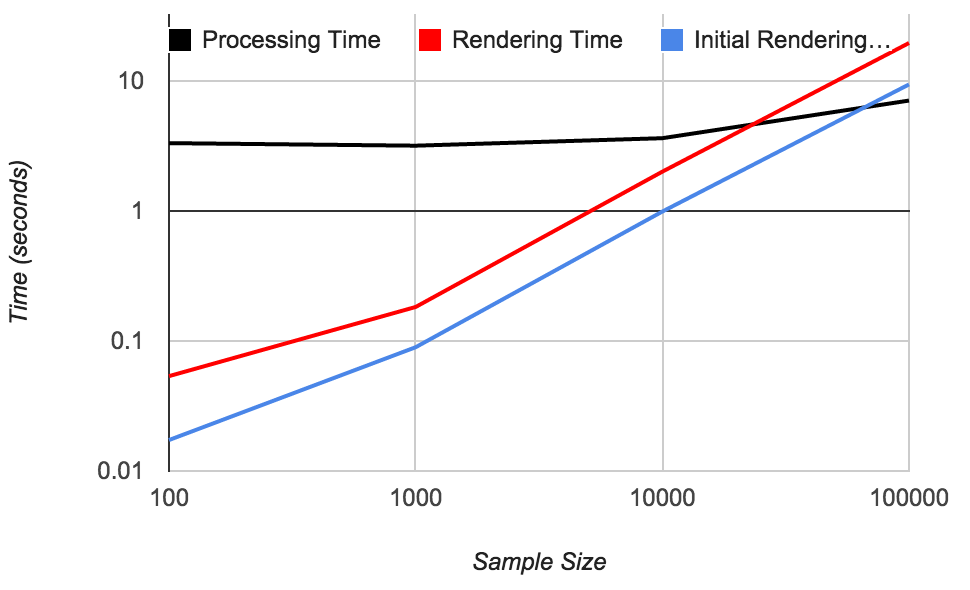
\includegraphics[width=3in]{figs/weather_perf.png}
\end{center}
\caption{Average processing and rendering time for local sampling data set.  Both axes are on a log scale.}\label{fig:weather_perf}
\end{figure}

The results of this experiment are presented in Figure \ref{fig:weather_perf}.
Interestingly, the processing time is nearly constant and only increases  at a sample size of 100,000.
The rendering time is approximately linear and faster than processing time until 100,000 records.
An interesting discovery is that the initial rendering time, the time it takes to render the plots using the initial sample, is consistently about half the time of the resampling rendering time.
This is likely due to the plots having to clear the plots before rendering on resample renders.
Thus, the total sampling and rendering time is about 5-10 seconds.
This can be considered acceptable as it will only be time taken for new points to show up when zooming.

\subsection{Remote Backend}

After evaluating the performance of a local data provider the performance of the remote back powered by Apache Spark and REST API described in Section \ref{sec:big_data_remote} is evaluated.  
To ensure comparability, a larger cut of the NOAA weather data with the same dashboard design is tested.

A Spark cluster consisting of 15 nodes with 16 cores per node and 20 GB of ram per node was used for the test.
The file was partitioned into 960 partitions (4 per core).
Prior to the experiments, a count of number of rows in the data set was performed and the data was cached.
This took about 1 minute of processing time but would only have to be done once assuming the cluster has sufficient memory to hold the dataset.

The larger weather dataset was similar to the local version; however, it contained weather from the whole world to get 300 million temperature measurements (about 100x larger than the local version).  
The data set was approximately 2 GB after processing.
A similar experiment as before was conducted; however, the remote dataset introduced additional processing times to measure.
In particular, the amount of time Spark spent processing the data and the total processing time as seen by iDcDashboard were both measured independently.

\begin{figure}
\begin{center}
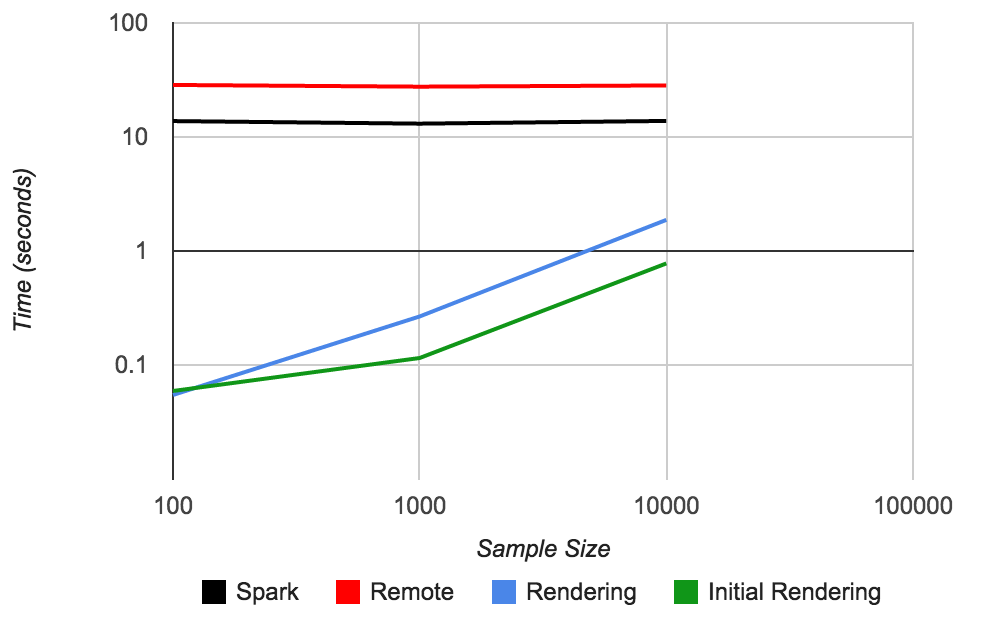
\includegraphics[width=3in]{figs/weather_big_perf.png}
\end{center}
\caption{Average processing and rendering time for remote sampling weather data set.  Both axes are on a log scale}\label{fig:weather_big_perf}
\end{figure}

The results of this experiment are presented in Figure \ref{fig:weather_big_perf}.
Sampling time and Spark execution time are constant, which matches results on the local machine;
however, interestingly Spark execution time accounts for only one half of the total sampling time.  
This is probably caused by network latency between the spark cluster to the web server and the websever to the iPython Notebook.
Rendering times are similar to local rendering time which is expected since the same dashboard was used and the backend has no impact on the rendering other than the data format (which is nearly the same).
Usability of the rendered dashboard was also the same as for the local case as expected.
A 30 second round trip time may be acceptable if hidden with the proposed multi-leveled cache system; however, it is much too slow to function as the sole data source (i.e. without iPython caching datasets).

\section{Conclusion}\label{sec:conclusion}%0.5 pages

In this paper the iDcDashboard, a novel system for exploratory visual analysis, is introduced.
Future work will concern the use of this system to visualize data streams in an efficient manner and to utilize this system for human guided machine learning.

This system was constructed over the Fall quarter of 2014 as David Lisuk's Master's research project.
I would like to thank Professor Yoav Freund for advising me throughout this project, Julaiti Alafate for assisting with the administration of the Spark cluster and providing ideas, and my girlfriend Stephanie Lum for supporting me through life in graduate school.

\bibliography{bib}
\onecolumn

\section{Appendix}
\centering
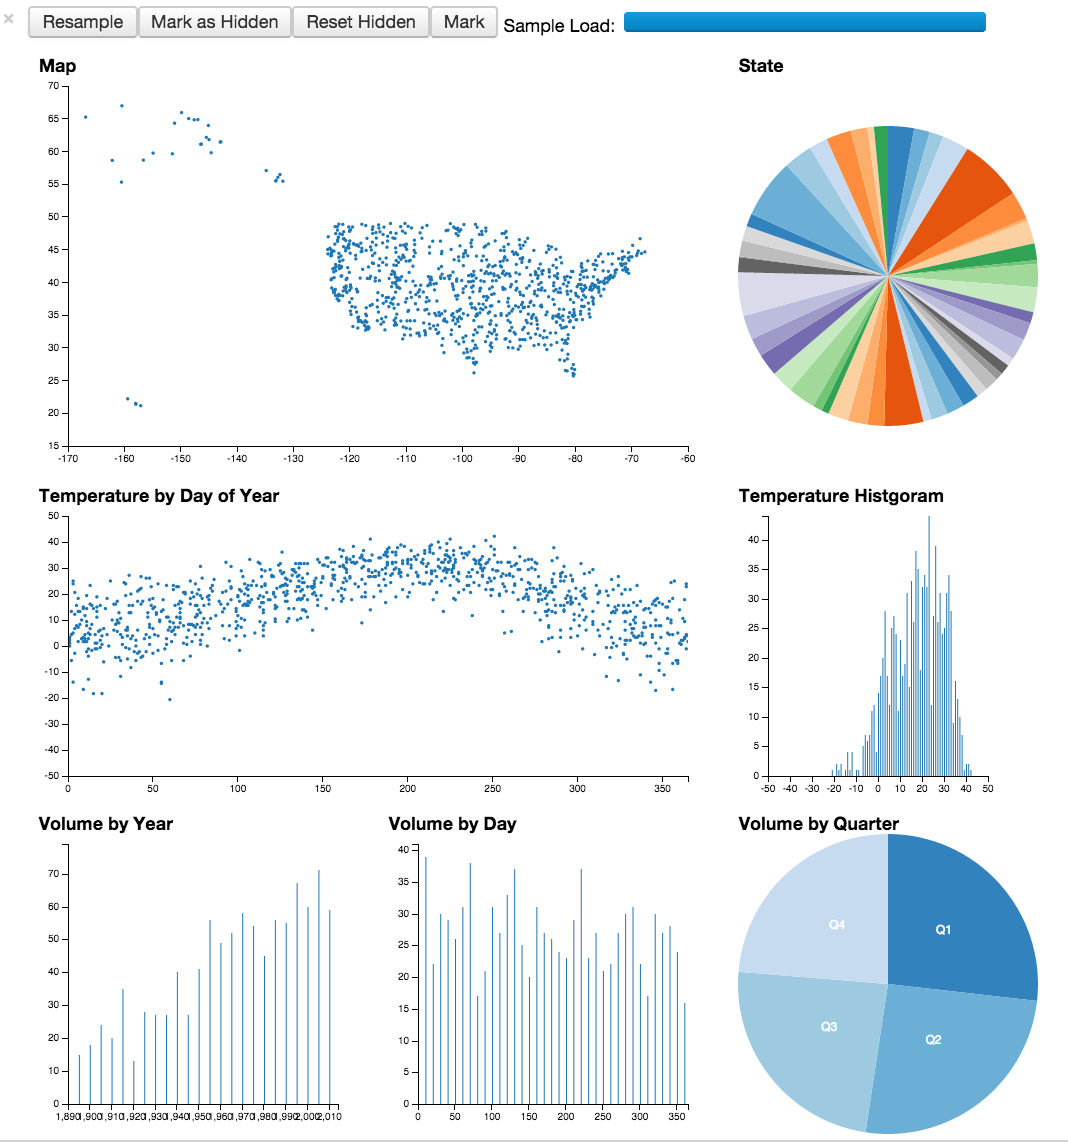
\includegraphics[width=6in]{figs/weather_dashboard.png}
\captionof{figure}{Screenshot of weather dashboard used in performance evaluations}\label{fig:weather}

\end{document}